\chapter{Исследовательская часть}

В данной части будет проведен анализ времени отрисовки кадра при различных входных данных.

\section{Технические характеристики}

Технические характеристики устройства, на котором выполнялся эксперимент представлены далее:

\begin{enumerate}[label=\arabic*)]
	\item операционная система --- Ubuntu 22.04.3~\cite{ubuntu} Linux x86\_64;
	\item память --- 16 Гб;
	\item процессор --- Intel® Core™ i5-1135G7 @ 2.40 ГГц.
\end{enumerate}

\section{Время генерации кадра}

Как было сказано выше, используются функции замера процессорного времени \textit{$std::chrono::system\_clock::now(...)$} и \textit{$std::chrono::duration\_cast<std::chrono::milliseconds>$} из библиотеки $chrono$ на \textit{C++}. Функция возвращает процессорное время в миллисекундах.

Функция используется дважды: перед началом отрисовки кадра и после завершения, затем из конечного времени вычитается начальное, чтобы получить результат.

Замеры проводились для разного количества фламинго на сцене --- от 1 до 15 и для разного количества источников света --- от 1 до 10.

Результаты замеров времени приведены в таблцицах \ref{tbl:time_flam} и \ref{tbl:time_lights}. А их графическое представление на рисунках \ref{fig:flams} и \ref{fig:lights} соответсвенно.

\begin{table}[h]
	\begin{center}
	\captionsetup{justification=raggedright,singlelinecheck=off}
	\caption{Результаты замеров времени для разного количества фламинго}
	\label{tbl:time_flam}
	\begin{tabular}{|c|r|}
		\hline
		кол-во фламинго & Время (в мс) \\
		\hline
		1 & 345.80 \\ 
		\hline
		2 & 392.48 \\ 
		\hline
		3 & 418.35 \\ 
		\hline
		4 & 436.24 \\ 
		\hline
		5 & 452.42 \\ 
		\hline
		6 & 473.84 \\ 
		\hline
		7 & 488.58 \\ 
		\hline
		8 & 504.36 \\ 
		\hline
		9 & 526.14 \\ 
		\hline
		10 & 553.01 \\ 
		\hline
		11 & 577.60 \\ 
		\hline
		12 & 621.60 \\ 
		\hline
		13 & 650.46 \\ 
		\hline
		14 & 666.34 \\ 
		\hline
		15 & 682.21 \\ 
		\hline
	\end{tabular}
\end{center}
\end{table}

\begin{table}[h]
	\begin{center}
		\captionsetup{justification=raggedright,singlelinecheck=off}
		\caption{Результаты замеров времени для разного количества источников света}
		\label{tbl:time_lights}
		\begin{tabular}{|c|r|}
			\hline
			кол-во источников света & Время (в мс) \\
			\hline
			1 & 370.90 \\ 
			\hline
			2 & 588.99 \\ 
			\hline
			3 & 772.40 \\ 
			\hline
			4 & 942.64 \\ 
			\hline
			5 & 1135.56 \\ 
			\hline
			6 & 1308.96 \\ 
			\hline
			7 & 1574.50 \\ 
			\hline
			8 & 1815.35 \\ 
			\hline
			9 & 2040.43 \\ 
			\hline
			10 & 2273.54 \\ 
			\hline
		\end{tabular}
	\end{center}
\end{table}

\begin{figure}[h!]
	\centering
	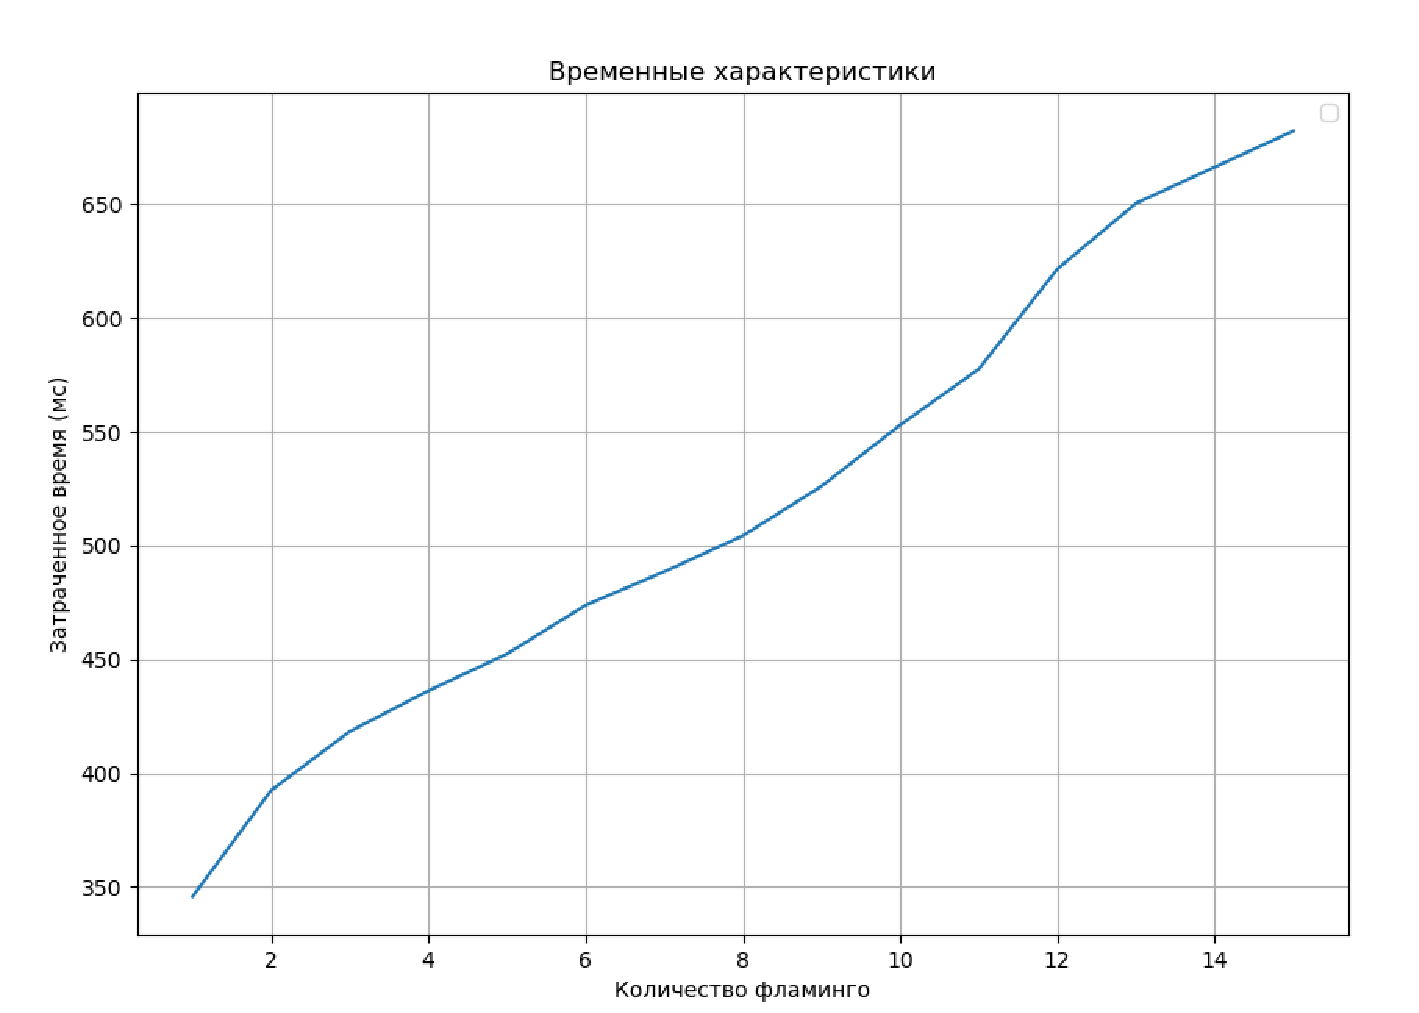
\includegraphics[width=0.9\linewidth]{img/flams}
	\caption{Сравнение времени отрисовки кадра для разного количества фламинго}
	\label{fig:flams}
\end{figure}

\begin{figure}[h!]
	\centering
	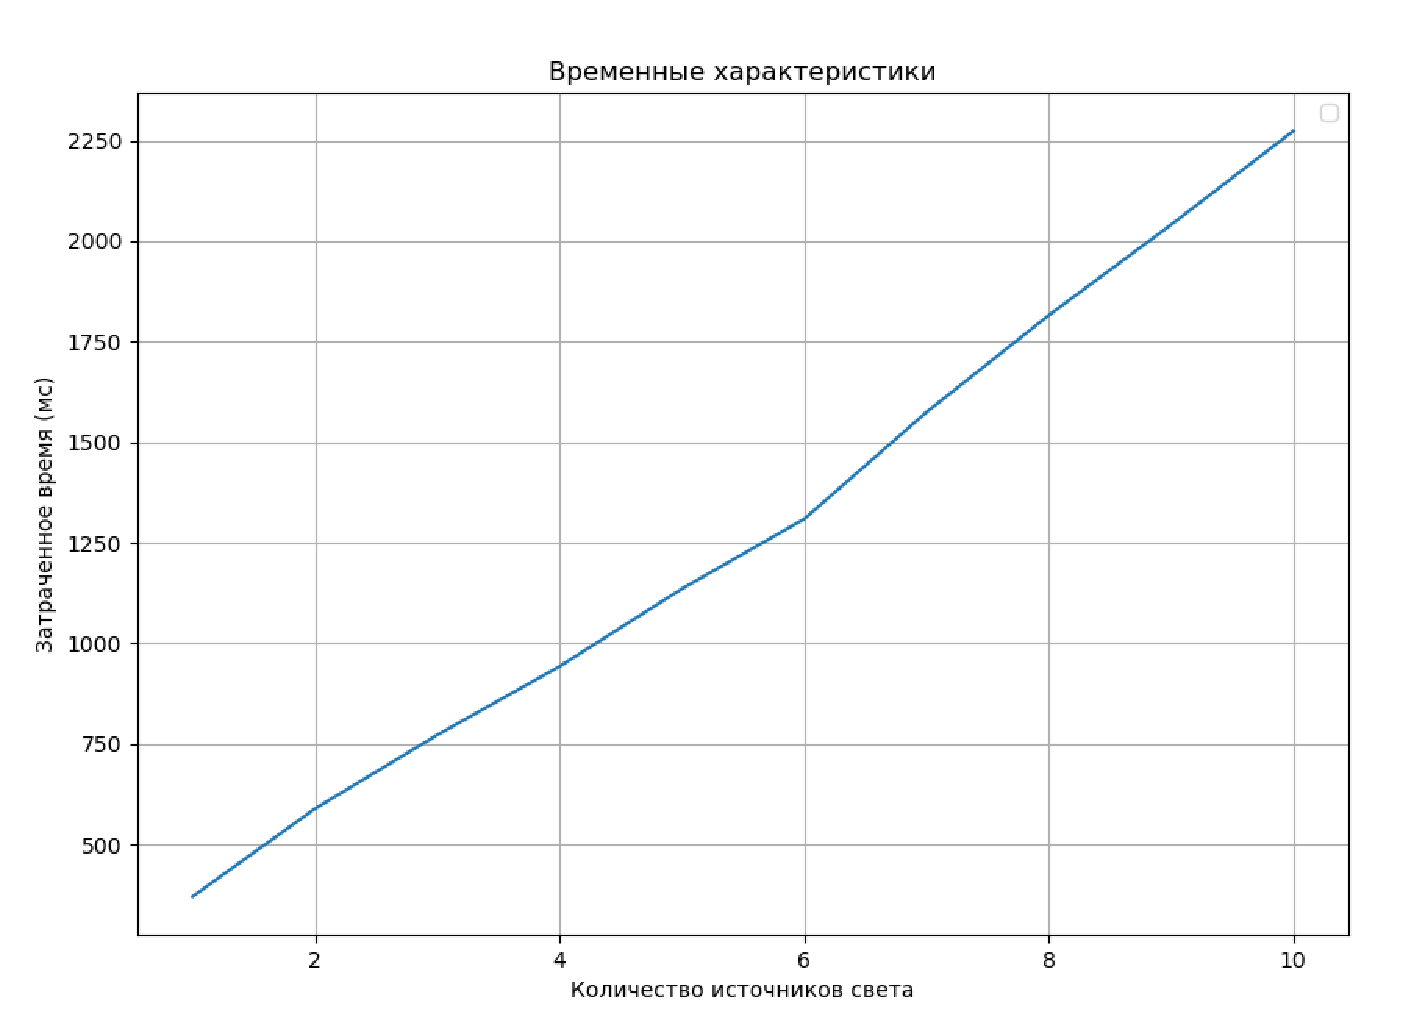
\includegraphics[width=0.9\linewidth]{img/lights}
	\caption{Сравнение времени отрисовки кадра для разного количества источников света}
	\label{fig:lights}
\end{figure}
\clearpage

\section*{Вывод}

В данной части был проведен сравнительный анализ времени выполнения работы программы для отрисовки 1 кадра при различном количестве фламинго и источников света на сцене. Из проведенного эксперимента можно сделать вывод, что функции зависимости времени и от количества фламинго, и от количества источников света на сцене --- линейны. В среднем на отрисовку кадра с 1 источником света требуется около 0.5 секунды, при количестве фламинго до 15.